\documentclass[]{article}
\usepackage{lmodern}
\usepackage{amssymb,amsmath}
\usepackage{ifxetex,ifluatex}
\usepackage{fixltx2e} % provides \textsubscript
\ifnum 0\ifxetex 1\fi\ifluatex 1\fi=0 % if pdftex
  \usepackage[T1]{fontenc}
  \usepackage[utf8]{inputenc}
\else % if luatex or xelatex
  \ifxetex
    \usepackage{mathspec}
  \else
    \usepackage{fontspec}
  \fi
  \defaultfontfeatures{Ligatures=TeX,Scale=MatchLowercase}
\fi
% use upquote if available, for straight quotes in verbatim environments
\IfFileExists{upquote.sty}{\usepackage{upquote}}{}
% use microtype if available
\IfFileExists{microtype.sty}{%
\usepackage{microtype}
\UseMicrotypeSet[protrusion]{basicmath} % disable protrusion for tt fonts
}{}
\usepackage[margin=1in]{geometry}
\usepackage{hyperref}
\hypersetup{unicode=true,
            pdftitle={Homework 4},
            pdfborder={0 0 0},
            breaklinks=true}
\urlstyle{same}  % don't use monospace font for urls
\usepackage{color}
\usepackage{fancyvrb}
\newcommand{\VerbBar}{|}
\newcommand{\VERB}{\Verb[commandchars=\\\{\}]}
\DefineVerbatimEnvironment{Highlighting}{Verbatim}{commandchars=\\\{\}}
% Add ',fontsize=\small' for more characters per line
\usepackage{framed}
\definecolor{shadecolor}{RGB}{248,248,248}
\newenvironment{Shaded}{\begin{snugshade}}{\end{snugshade}}
\newcommand{\KeywordTok}[1]{\textcolor[rgb]{0.13,0.29,0.53}{\textbf{#1}}}
\newcommand{\DataTypeTok}[1]{\textcolor[rgb]{0.13,0.29,0.53}{#1}}
\newcommand{\DecValTok}[1]{\textcolor[rgb]{0.00,0.00,0.81}{#1}}
\newcommand{\BaseNTok}[1]{\textcolor[rgb]{0.00,0.00,0.81}{#1}}
\newcommand{\FloatTok}[1]{\textcolor[rgb]{0.00,0.00,0.81}{#1}}
\newcommand{\ConstantTok}[1]{\textcolor[rgb]{0.00,0.00,0.00}{#1}}
\newcommand{\CharTok}[1]{\textcolor[rgb]{0.31,0.60,0.02}{#1}}
\newcommand{\SpecialCharTok}[1]{\textcolor[rgb]{0.00,0.00,0.00}{#1}}
\newcommand{\StringTok}[1]{\textcolor[rgb]{0.31,0.60,0.02}{#1}}
\newcommand{\VerbatimStringTok}[1]{\textcolor[rgb]{0.31,0.60,0.02}{#1}}
\newcommand{\SpecialStringTok}[1]{\textcolor[rgb]{0.31,0.60,0.02}{#1}}
\newcommand{\ImportTok}[1]{#1}
\newcommand{\CommentTok}[1]{\textcolor[rgb]{0.56,0.35,0.01}{\textit{#1}}}
\newcommand{\DocumentationTok}[1]{\textcolor[rgb]{0.56,0.35,0.01}{\textbf{\textit{#1}}}}
\newcommand{\AnnotationTok}[1]{\textcolor[rgb]{0.56,0.35,0.01}{\textbf{\textit{#1}}}}
\newcommand{\CommentVarTok}[1]{\textcolor[rgb]{0.56,0.35,0.01}{\textbf{\textit{#1}}}}
\newcommand{\OtherTok}[1]{\textcolor[rgb]{0.56,0.35,0.01}{#1}}
\newcommand{\FunctionTok}[1]{\textcolor[rgb]{0.00,0.00,0.00}{#1}}
\newcommand{\VariableTok}[1]{\textcolor[rgb]{0.00,0.00,0.00}{#1}}
\newcommand{\ControlFlowTok}[1]{\textcolor[rgb]{0.13,0.29,0.53}{\textbf{#1}}}
\newcommand{\OperatorTok}[1]{\textcolor[rgb]{0.81,0.36,0.00}{\textbf{#1}}}
\newcommand{\BuiltInTok}[1]{#1}
\newcommand{\ExtensionTok}[1]{#1}
\newcommand{\PreprocessorTok}[1]{\textcolor[rgb]{0.56,0.35,0.01}{\textit{#1}}}
\newcommand{\AttributeTok}[1]{\textcolor[rgb]{0.77,0.63,0.00}{#1}}
\newcommand{\RegionMarkerTok}[1]{#1}
\newcommand{\InformationTok}[1]{\textcolor[rgb]{0.56,0.35,0.01}{\textbf{\textit{#1}}}}
\newcommand{\WarningTok}[1]{\textcolor[rgb]{0.56,0.35,0.01}{\textbf{\textit{#1}}}}
\newcommand{\AlertTok}[1]{\textcolor[rgb]{0.94,0.16,0.16}{#1}}
\newcommand{\ErrorTok}[1]{\textcolor[rgb]{0.64,0.00,0.00}{\textbf{#1}}}
\newcommand{\NormalTok}[1]{#1}
\usepackage{graphicx,grffile}
\makeatletter
\def\maxwidth{\ifdim\Gin@nat@width>\linewidth\linewidth\else\Gin@nat@width\fi}
\def\maxheight{\ifdim\Gin@nat@height>\textheight\textheight\else\Gin@nat@height\fi}
\makeatother
% Scale images if necessary, so that they will not overflow the page
% margins by default, and it is still possible to overwrite the defaults
% using explicit options in \includegraphics[width, height, ...]{}
\setkeys{Gin}{width=\maxwidth,height=\maxheight,keepaspectratio}
\IfFileExists{parskip.sty}{%
\usepackage{parskip}
}{% else
\setlength{\parindent}{0pt}
\setlength{\parskip}{6pt plus 2pt minus 1pt}
}
\setlength{\emergencystretch}{3em}  % prevent overfull lines
\providecommand{\tightlist}{%
  \setlength{\itemsep}{0pt}\setlength{\parskip}{0pt}}
\setcounter{secnumdepth}{0}
% Redefines (sub)paragraphs to behave more like sections
\ifx\paragraph\undefined\else
\let\oldparagraph\paragraph
\renewcommand{\paragraph}[1]{\oldparagraph{#1}\mbox{}}
\fi
\ifx\subparagraph\undefined\else
\let\oldsubparagraph\subparagraph
\renewcommand{\subparagraph}[1]{\oldsubparagraph{#1}\mbox{}}
\fi

%%% Use protect on footnotes to avoid problems with footnotes in titles
\let\rmarkdownfootnote\footnote%
\def\footnote{\protect\rmarkdownfootnote}

%%% Change title format to be more compact
\usepackage{titling}

% Create subtitle command for use in maketitle
\newcommand{\subtitle}[1]{
  \posttitle{
    \begin{center}\large#1\end{center}
    }
}

\setlength{\droptitle}{-2em}

  \title{Homework 4}
    \pretitle{\vspace{\droptitle}\centering\huge}
  \posttitle{\par}
    \author{}
    \preauthor{}\postauthor{}
    \date{}
    \predate{}\postdate{}
  

\begin{document}
\maketitle

\bigskip

(For questions \textbf{1, 2}) The following data show the liver weights
(kg) taken from randomly selected cattle in two farms in southwest
England during outbreaks of liver fluke disease.

\begin{Shaded}
\begin{Highlighting}[]
\NormalTok{farm1 <-}\StringTok{ }\KeywordTok{c}\NormalTok{(}\FloatTok{18.0}\NormalTok{, }\FloatTok{18.5}\NormalTok{, }\FloatTok{18.9}\NormalTok{, }\FloatTok{18.2}\NormalTok{, }\FloatTok{17.9}\NormalTok{, }\FloatTok{15.9}\NormalTok{, }\FloatTok{16.8}\NormalTok{, }\FloatTok{18.2}\NormalTok{, }\FloatTok{17.3}\NormalTok{, }\FloatTok{17.5}\NormalTok{, }\FloatTok{17.7}\NormalTok{, }\FloatTok{17.8}\NormalTok{, }\FloatTok{17.1}\NormalTok{,}
           \FloatTok{17.0}\NormalTok{, }\FloatTok{16.3}\NormalTok{)}
\NormalTok{farm2 <-}\StringTok{ }\KeywordTok{c}\NormalTok{(}\FloatTok{14.3}\NormalTok{, }\FloatTok{13.2}\NormalTok{, }\FloatTok{17.3}\NormalTok{, }\FloatTok{14.9}\NormalTok{, }\FloatTok{16.4}\NormalTok{, }\FloatTok{16.0}\NormalTok{, }\FloatTok{18.6}\NormalTok{, }\FloatTok{17.3}\NormalTok{, }\FloatTok{15.5}\NormalTok{, }\FloatTok{16.8}\NormalTok{, }\FloatTok{15.7}\NormalTok{, }\FloatTok{18.0}\NormalTok{, }\FloatTok{15.2}\NormalTok{)}
\end{Highlighting}
\end{Shaded}

\textbf{1.} (a) Create the following data frame:

\begin{verbatim}
##     farm liver_weight
## 1  farm1         18.0
## 2  farm1         18.5
## 3  farm1         18.9
## 4  farm1         18.2
## 5  farm1         17.9
## 6  farm1         15.9
## 7  farm1         16.8
## 8  farm1         18.2
## 9  farm1         17.3
## 10 farm1         17.5
## 11 farm1         17.7
## 12 farm1         17.8
## 13 farm1         17.1
## 14 farm1         17.0
## 15 farm1         16.3
## 16 farm2         14.3
## 17 farm2         13.2
## 18 farm2         17.3
## 19 farm2         14.9
## 20 farm2         16.4
## 21 farm2         16.0
## 22 farm2         18.6
## 23 farm2         17.3
## 24 farm2         15.5
## 25 farm2         16.8
## 26 farm2         15.7
## 27 farm2         18.0
## 28 farm2         15.2
\end{verbatim}

\begin{enumerate}
\def\labelenumi{(\alph{enumi})}
\setcounter{enumi}{1}
\tightlist
\item
  Using \texttt{group\_by()} and \texttt{summarize()} combination,
  create the following summary table:
\end{enumerate}

\begin{verbatim}
## # A tibble: 2 x 3
##   farm  sample_mean sample_var
##   <fct>       <dbl>      <dbl>
## 1 farm1        17.5      0.671
## 2 farm2        16.1      2.31
\end{verbatim}

\textbf{2.} (a) As a preliminary to testing the null hypothesis that the
mean liver weights of the cattle in the two farms are the same, check if
the population variances in the two farms can be assumed to be similar.

\begin{enumerate}
\def\labelenumi{(\alph{enumi})}
\setcounter{enumi}{1}
\tightlist
\item
  Use an appropriate test to check if \texttt{farm1} population mean is
  the same as \texttt{farm2} population mean.
\end{enumerate}

(For questions \textbf{3, 4}), In the following, the measurements of the
mean fluorescence intensity of sperm cells stained with a fluorescent
marker, 1-anilinonaphthalene-8-sulphonate (ANS), showing the effect of
the presence of egg yolk in the diluent solution. ANS fluoresces only
when bound to the sperm membrane. Each value represents the mean of 10
individual spermatozoa and is estimated by a densitometer from
photographic film.

\begin{Shaded}
\begin{Highlighting}[]
\NormalTok{egg_yolk_1_percent <-}\StringTok{ }\KeywordTok{c}\NormalTok{(}\FloatTok{0.944}\NormalTok{, }\FloatTok{1.048}\NormalTok{, }\FloatTok{1.026}\NormalTok{, }\FloatTok{1.007}\NormalTok{, }\FloatTok{0.933}\NormalTok{, }\FloatTok{0.998}\NormalTok{, }\FloatTok{1.035}\NormalTok{)}
\NormalTok{egg_yolk_5_percent <-}\StringTok{ }\KeywordTok{c}\NormalTok{(}\FloatTok{0.865}\NormalTok{, }\FloatTok{1.000}\NormalTok{, }\FloatTok{1.001}\NormalTok{, }\FloatTok{0.900}\NormalTok{, }\FloatTok{0.923}\NormalTok{, }\FloatTok{0.876}\NormalTok{, }\FloatTok{1.046}\NormalTok{, }\FloatTok{0.990}\NormalTok{)}
\NormalTok{egg_yolk_25_percent <-}\StringTok{ }\KeywordTok{c}\NormalTok{(}\FloatTok{0.811}\NormalTok{, }\FloatTok{0.862}\NormalTok{, }\FloatTok{0.910}\NormalTok{, }\FloatTok{0.799}\NormalTok{, }\FloatTok{0.837}\NormalTok{, }\FloatTok{0.854}\NormalTok{)}
\end{Highlighting}
\end{Shaded}

\textbf{3.} (a) Create the following box plot:

\begin{center}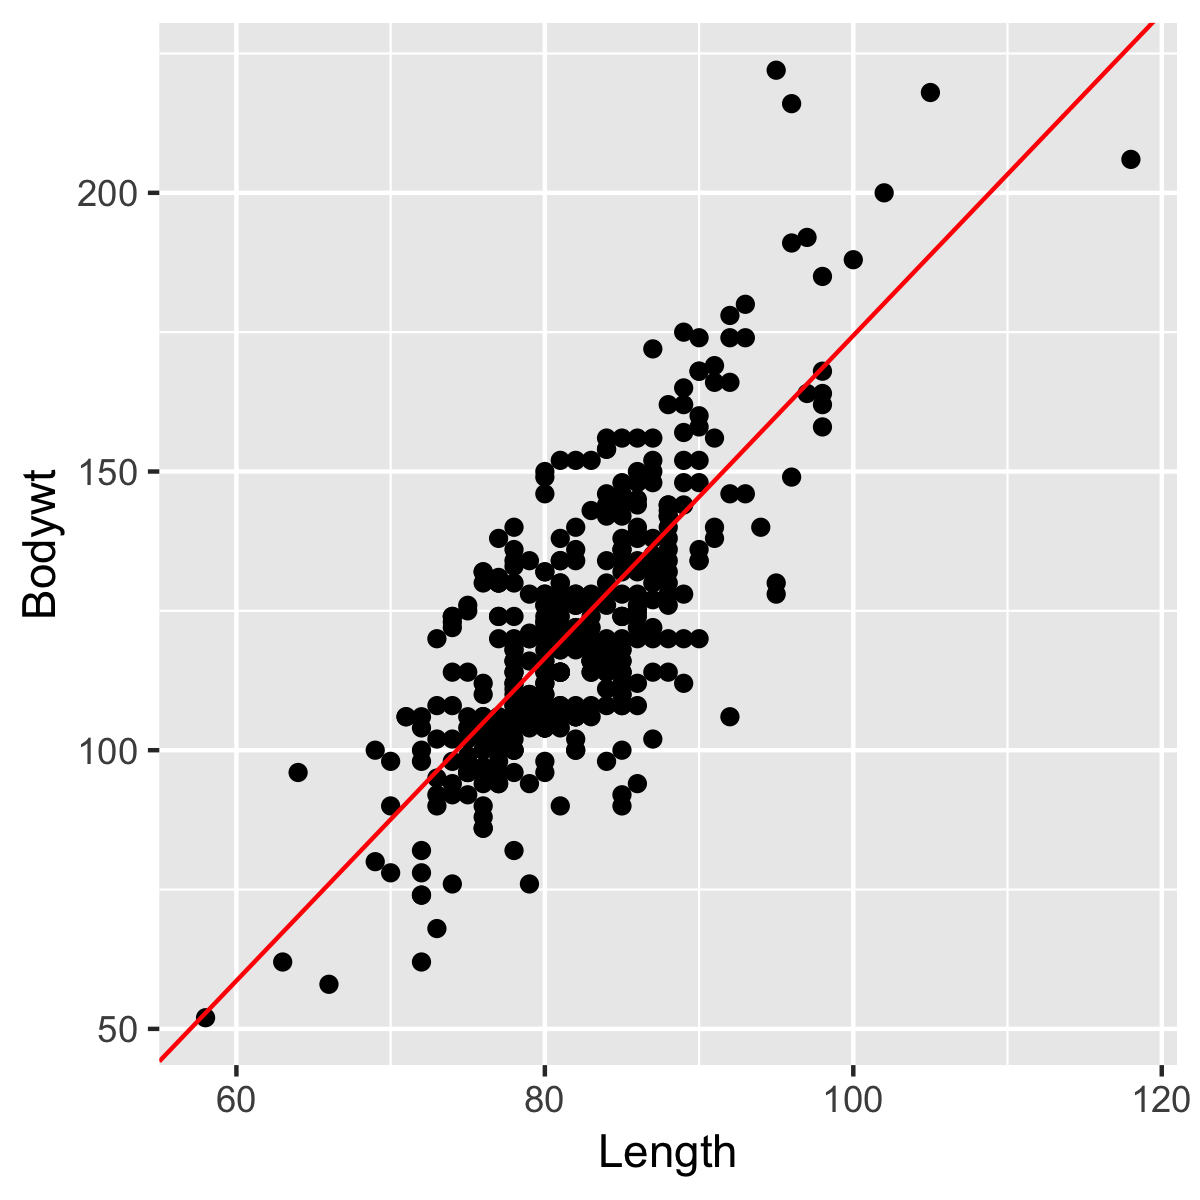
\includegraphics{HW4_files/figure-latex/unnamed-chunk-7-1} \end{center}

\begin{enumerate}
\def\labelenumi{(\alph{enumi})}
\setcounter{enumi}{1}
\tightlist
\item
  What evidence is there that the egg yolk percentage affects the
  fluorescence intensity of sperm cells? Use an appropriate test to
  support your answer. You may assume that the population variances of
  the intensity in each group are the same.
\end{enumerate}

\textbf{4.} Based on the result from \textbf{3} (b) above, perform post
hoc analyses, that is, determine which pair(s) of percentages, if any,
shows difference in fluorescence intensity.

\textbf{5.} Out of 183 female Beagles, 120 randomly selected dogs were
given 0.026-106 kBq plutonium per kg by intravenous injection and
compared with remaining 63 female control dogs with a view to
determining whether plutonium deposit in bone affects the appearance of
mammary tumors. 45 of the control dogs developed mammary tumors of any
kind whereas 67 of the dogs given plutonium developed mammary tumors of
any kind. The following is a \(2\times 2\) contingency table describing
the outcome:

\[\begin{array}{c|ccc} & \text{Plutonium} & \text{Control} & \text{Total} \\ \hline   
\text{Tumor} & 67 & 45 & 112 \\  
\text{No tumor} & 53 & 18 & 71 \\
\text{Total} & 120 & 63 & 183
\end{array}\]

Using \(\chi^2\)-test \emph{with Yates' correction}, determine whether
tumor development is associated with plutonium deposit in bone.


\end{document}
